% Reviewer-ready replacement for the current Section 3.2.
% The goal is to address the reviewers' concerns by separating
% (i) derivative-level quadrature validation,
% (ii) implementation-level floating-point diagnostics,
% (iii) cutoff trade-off checks, and
% (iv) asymptotic convergence-rate evidence.

\subsection{Derivative-level validation and implementation diagnostics}
\label{subsec:num-valid}

This subsection provides derivative-level numerical evidence for the quadrature and implementation consequences of the analysis in Section~3.  The identities and stability estimates in Theorems~\ref{thm:represent_2}--\ref{thm:stability} are already established analytically; the goal here is not to reprove them by experiment.  Instead, the tests below isolate four effects that enter practical implementations of the estimators in Corollary~\ref{coro:4}: Monte Carlo sampling error, Gauss--Jacobi quadrature error, denominator regularization error, and finite-precision cancellation in endpoint difference quotients.  These are derivative-evaluation tests rather than PINN training experiments, so that quadrature effects are not confounded with neural-network approximation or optimization errors.

Unless otherwise stated, the smooth benchmark is
\begin{equation}
    f(t)=e^{-t},\qquad t=1.5,
    \label{eq:valid-exp-benchmark}
\end{equation}
for which
\begin{equation}
    \partial_t^\alpha f(t)=t^{2-\alpha}E_{1,3-\alpha}(-t).
\end{equation}
Monte Carlo samples are drawn from $\mathrm{Beta}(2-\alpha,1)$, and Gauss--Jacobi nodes and weights are computed for the weight $\tau^{1-\alpha}$ on $[0,1]$.  Unless explicitly stated otherwise, errors are relative derivative errors,
\begin{equation}
    \mathrm{err}=\frac{\abs{\partial_t^\alpha f(t)-\bar\partial_\tau^\alpha f(t)}}{\abs{\partial_t^\alpha f(t)}}.
\end{equation}

We distinguish carefully between \emph{raw} and \emph{stable} quotient evaluations.  For the exponential benchmark, with $h=t\tau$, the raw kernels are
\begin{equation}
K_f(t,\tau)=\frac{f'(t)-f'(t-h)}{h},\qquad
H_f(t,\tau)=\frac{f(t)-f(t-h)-h f'(t)}{h^2}.
\end{equation}
Their stable algebraic forms are evaluated as
\begin{equation}
    K_f^{\rm stab}(t,\tau)=e^{-t}\frac{\operatorname{expm1}(h)}{h},
    \qquad
    H_f^{\rm stab}(t,\tau)=e^{-t}\frac{h-\operatorname{expm1}(h)}{h^2},
    \label{eq:valid-stable-exp}
\end{equation}
with Taylor endpoint replacement when $h$ is below machine-resolution thresholds:
\begin{equation}
    K_f(t,0)=e^{-t},
    \qquad
    H_f(t,0)=-\frac12e^{-t}.
\end{equation}
This definition is important: Lemma~\ref{lem:type-kernels} removes the endpoint singularity at the continuous level, but a raw floating-point quotient need not evaluate that removable singularity accurately.

\paragraph*{Dependence on the fractional order.}
For Monte Carlo sampling, the endpoint mass is explicit:
\begin{equation}
    \mathbb P(\tau<\varepsilon/t)=(\varepsilon/t)^{2-\alpha},
    \qquad \tau\sim \mathrm{Beta}(2-\alpha,1).
    \label{eq:valid-endpoint-mass}
\end{equation}
Thus, as $\alpha\to2$, a larger fraction of samples falls in the interval where raw quotient evaluation and denominator regularization are most exposed to endpoint perturbations.  Figure~\ref{fig:valid-alpha} shows this behavior.  The Monte Carlo curves deteriorate near $\alpha=2$, whereas the Gauss--Jacobi rules remain near machine precision for the smooth benchmark when stable endpoint evaluation is used.  This should not be interpreted as a failure of the $M^{-1/2}$ Monte Carlo rate in Proposition~\ref{prop:mc-convergence}; rather, it shows that the practical regularized/raw estimator becomes increasingly endpoint-sensitive near the second-order limit.

\begin{figure}[htbp]
    \centering
    
\includegraphics[width=0.92\textwidth]{figures/fig_valid_alpha_sweep_exp.pdf}
    \caption{Derivative-level sensitivity with respect to $\alpha$ for the benchmark \eqref{eq:valid-exp-benchmark}.  The right panel reports the endpoint mass \eqref{eq:valid-endpoint-mass}.  The deterioration of the Monte Carlo curves near $\alpha=2$ is consistent with increased endpoint exposure of the practical estimator, not with a change of the theoretical Monte Carlo rate.}
    \label{fig:valid-alpha}
\end{figure}

\paragraph*{Dependence on quadrature size and the role of endpoint cancellation.}
The quadrature-size experiment separates stochastic sampling error from floating-point cancellation.  For Monte Carlo, repeated runs show decreasing median error as $M$ grows, although individual runs are not monotone.  For instance, for $\alpha=1.5$ and the benchmark \eqref{eq:valid-exp-benchmark}, the MC-II median relative error decreases from $1.35\times10^{-2}$ at $M=10$ to $2.24\times10^{-4}$ at $M=10240$; see Table~\ref{tab:valid-M-effect}.  This agrees with the statistical behavior predicted by Proposition~\ref{prop:mc-convergence}.

For Gauss--Jacobi quadrature, increasing $M$ has a different practical effect.  The mathematical quadrature error decreases rapidly for smooth kernels, but the leftmost Jacobi node approaches the endpoint at the scale $\tau_{\min}=O(M^{-2})$ for fixed Jacobi parameters.  Hence large $M$ exposes raw quotients to smaller endpoint denominators.  The continuous singularity is removable, but the raw forms subtract nearly equal numbers and then divide by $\tau$ or $\tau^2$.  Figure~\ref{fig:valid-M} and Table~\ref{tab:valid-M-effect} show that the raw Type-II Gauss--Jacobi error can increase in the large-$M$ regime, while the stable quotient remains much more accurate.  This is an implementation-level cancellation effect, not a deterioration of the Gauss--Jacobi quadrature rule itself.

\begin{table}[htbp]
\centering
\caption{Representative quadrature-size effects for $f(t)=e^{-t}$, $t=1.5$, and $\alpha=1.5$.  The Monte Carlo columns report median relative errors over repeated runs.  The Gauss--Jacobi columns compare raw and stable Type-II quotient evaluations.}
\label{tab:valid-M-effect}
\begin{tabular}{c|cc|ccc}
\hline
$M$ & MC-I median & MC-II median & $\tau_{\min}$ & GJ-II raw & GJ-II stable \\
\hline
$10$    & $2.67\times10^{-2}$ & $1.35\times10^{-2}$ & $5.86\times10^{-3}$ & $1.40\times10^{-13}$ & $7.84\times10^{-16}$ \\
$80$    & $7.19\times10^{-3}$ & $3.49\times10^{-3}$ & $9.58\times10^{-5}$ & $5.09\times10^{-11}$ & $1.67\times10^{-14}$ \\
$320$   & $4.07\times10^{-3}$ & $1.43\times10^{-3}$ & $6.01\times10^{-6}$ & $3.39\times10^{-9}$  & $3.37\times10^{-14}$ \\
$1280$  & $1.85\times10^{-3}$ & $1.01\times10^{-3}$ & $3.76\times10^{-7}$ & $8.66\times10^{-8}$  & $2.36\times10^{-12}$ \\
$10240$ & $8.85\times10^{-4}$ & $2.24\times10^{-4}$ & -- & -- & -- \\
\hline
\end{tabular}
\end{table}

\begin{figure}[htbp]
    \centering
    
\includegraphics[width=0.92\textwidth]{figures/fig_valid_M_sweep_exp_diagnostic.pdf}
    \caption{Effect of the number of quadrature points $M$.  Left: repeated Monte Carlo runs show decreasing median errors with interquartile variability.  Middle: Gauss--Jacobi raw and stable quotients separate when endpoint cancellation dominates.  Right: $\tau_{\min}$ scales like $M^{-2}$, which explains why increasing $M$ may expose raw endpoint quotients to stronger cancellation.}
    \label{fig:valid-M}
\end{figure}

\paragraph*{Finite-precision diagnosis.}
The preceding observation motivates a direct finite-precision test of the raw quotients.  Figure~\ref{fig:valid-precision} compares fp64, fp32, fp16, and fp8-like quantized evaluations.  The fp8 curves should be interpreted only as controlled e5m2/e4m3-style quantization diagnostics for the scalar quotient kernels; they are not intended to reproduce a full hardware mixed-precision PINN training pipeline.  The result is nevertheless informative: Type-II is more sensitive than Type-I because its denominator scales as $(t\tau)^2$.  In low precision, the raw Type-II quotient reaches the endpoint-dominated regime much earlier.  This supports the practical recommendation to use stable quotient formulas, endpoint Taylor replacement, or moderate Gauss--Jacobi $M$ values when raw quotients are unavoidable.

\begin{figure}[htbp]
    \centering
    
\includegraphics[width=0.92\textwidth]{figures/fig_valid_precision_raw_quotients.pdf}
    \caption{Finite-precision diagnosis of raw endpoint quotients.  The reference is the stabilized fp64 quotient.  Type-II is more vulnerable to precision loss because the removable singularity is evaluated through a second-order denominator.  The fp8 curves are quantization diagnostics, not full mixed-precision training experiments.}
    \label{fig:valid-precision}
\end{figure}

% Suggested insertion for Section 3.2, after the alpha-sensitivity or finite-precision paragraph.

\paragraph*{Order-dependent finite-precision effect near $\alpha=2$.}
The preceding $\alpha$-sweep also reveals a subtle point: even for Gauss--Jacobi quadrature, the raw quotient error may increase as $\alpha\to2$.  To determine whether this behavior is due to the quadrature rule or to floating-point evaluation of the endpoint quotients, we repeat the Gauss--Jacobi $\alpha$-sweep for the smooth benchmark $f(t)=e^{-t}$, $t=1.5$, and $M=100$, while evaluating the raw quotients under fp64, fp32, fp16 and fp8-like quantization.  The fp8-like curves use e5m2/e4m3 quantization diagnostics and are not intended to model a complete mixed-precision training pipeline.

\begin{figure}[htbp]
    \centering
    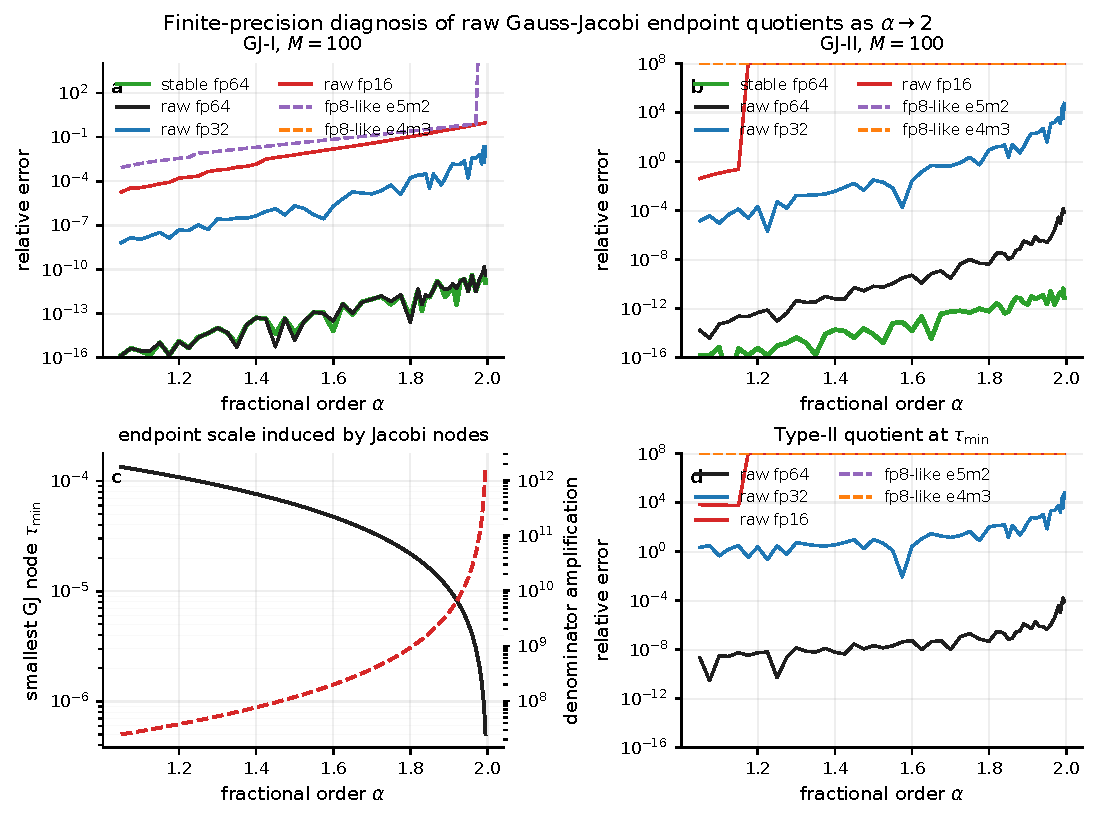
\includegraphics[width=0.95\textwidth]{figures/fig12_alpha2_gj_precision_sweep.pdf}
    \caption{Finite-precision diagnosis of raw Gauss--Jacobi endpoint quotients as $\alpha\to2$ for $f(t)=e^{-t}$, $t=1.5$, and $M=100$.  Stable fp64 uses algebraically equivalent \texttt{expm1}/Taylor endpoint formulas.  The raw fp64 Type-II error increases near $\alpha=2$, fp32 deteriorates much earlier, and fp16/fp8-like evaluations enter overflow or invalid regimes.  The lower-left panel shows that the leftmost node approaches $\tau=0$ as $\alpha\to2$, increasing the denominator amplification $(t\tau_{\min})^{-2}$.}
    \label{fig:valid-alpha2-precision}
\end{figure}

\begin{table}[htbp]
\centering
\caption{Relative GJ-II errors as $\alpha\to2$ under different quotient-evaluation precisions.  The final two columns report the relative error of the local Type-II quotient at the smallest Gauss--Jacobi node.  Values marked overflow/NaN indicate that the quantized denominator or numerator evaluation became invalid.}
\label{tab:valid-alpha2-precision}
\begin{tabular}{c|cc|ccccc|cc}
\hline
$\alpha$ & $\tau_{\min}$ & $(t\tau_{\min})^{-2}$ & stable fp64 & raw fp64 & raw fp32 & raw fp16 & fp8-like e5m2 & local q2 fp64 & local q2 fp32 \\
\hline
$1.25$ & $9.99\times10^{-5}$ & $4.46\times10^{7}$  & $9.61\times10^{-16}$ & $9.85\times10^{-14}$ & $5.30\times10^{-4}$ & overflow/NaN & overflow/NaN & $5.28\times10^{-11}$ & $2.93$ \\
$1.50$ & $6.14\times10^{-5}$ & $1.18\times10^{8}$  & $2.35\times10^{-15}$ & $6.89\times10^{-11}$ & $3.21\times10^{-2}$ & overflow/NaN & overflow/NaN & $2.19\times10^{-8}$  & $9.98$ \\
$1.75$ & $2.79\times10^{-5}$ & $5.69\times10^{8}$  & $1.12\times10^{-13}$ & $1.05\times10^{-8}$  & $2.33$              & overflow/NaN & overflow/NaN & $2.03\times10^{-7}$  & $4.49\times10^{1}$ \\
$1.90$ & $1.05\times10^{-5}$ & $4.05\times10^{9}$  & $2.16\times10^{-12}$ & $2.56\times10^{-7}$  & $6.81\times10^{1}$ & overflow/NaN & overflow/NaN & $8.70\times10^{-7}$  & $2.32\times10^{2}$ \\
$1.98$ & $2.02\times10^{-6}$ & $1.09\times10^{11}$ & $1.20\times10^{-11}$ & $2.93\times10^{-5}$  & $4.08\times10^{3}$ & overflow/NaN & overflow/NaN & $3.77\times10^{-5}$  & $5.25\times10^{3}$ \\
$1.99$ & $1.00\times10^{-6}$ & $4.40\times10^{11}$ & $1.19\times10^{-11}$ & $8.75\times10^{-5}$  & $2.96\times10^{4}$ & overflow/NaN & overflow/NaN & $9.93\times10^{-5}$  & $3.36\times10^{4}$ \\
\hline
\end{tabular}
\end{table}

\begin{remark}[Raw Gauss--Jacobi quotients near $\alpha=2$]
The increase of raw Gauss--Jacobi errors near $\alpha=2$ is an implementation-level finite-precision effect rather than a failure of the quadrature rule.  In the Type-II formula, the quotient
\[
    \frac{f(t)-f(t-h)-h f'(t)}{h^2},\qquad h=t\tau,
\]
forms an $O(h^2)$ numerator by subtracting $O(1)$ quantities and then divides by $h^2$.  As $\alpha\to2$, the Jacobi exponent $1-\alpha\to-1$, and the left endpoint nodes move closer to $\tau=0$.  Therefore, raw endpoint quotients become increasingly roundoff-sensitive.  For smooth benchmarks, this sensitivity is removed by algebraically stable endpoint evaluation, for example by using \texttt{expm1} and Taylor replacement near $h=0$.  Hence large errors from raw low-precision quotients should be interpreted as endpoint-cancellation artifacts, not as contradictions of the Gauss--Jacobi convergence theorem for exactly evaluated smooth kernels.
\end{remark}


\paragraph*{Cutoff bias--conditioning trade-off.}
We next perform an asymptotic numerical check of Remark~3.1.  This experiment is deliberately not presented as an independent PINN-training validation of the full error; instead, it evaluates the leading bias and conditioning components in Propositions~\ref{prop:delta-conditioning} and~\ref{prop:regularization-bias}.  The predicted powers are
\begin{equation}
    \text{regularization bias}:\quad \delta^{2-\alpha},
    \qquad
    A_\alpha(\delta),C_\alpha(\delta):\quad \delta^{1-\alpha},
    \qquad
    B_\alpha(\delta):\quad \delta^{-\alpha}.
\end{equation}
The test uses three representative fractional orders, $\alpha=1.25,1.50,1.75$.  The measured log--log slopes in Table~\ref{tab:valid-tradeoff-slopes} agree with the predicted exponents.  In particular, as $\alpha$ approaches $2$, the Type-II function-value perturbation term $B_\alpha(\delta)$ becomes increasingly singular; this quantifies why the admissible window for choosing the denominator cutoff narrows near the second-order limit.

\begin{table}[htbp]
\centering
\caption{Asymptotic check of the cutoff trade-off in Remark~3.1.  The measured slopes are obtained from the regularization-bias and conditioning-integral components in Propositions~\ref{prop:delta-conditioning}--\ref{prop:regularization-bias}.}
\label{tab:valid-tradeoff-slopes}
\begin{tabular}{c|cc|ccc|cc|cc}
\hline
$\alpha$ & bias exp. & measured & $A,C$ exp. & $A$ & $C$ & $B$ exp. & $B$ & $\delta_*^I$ & $\delta_*^{II}$ \\
\hline
1.25 & 0.75 & 0.75 & -0.25 & -0.25 & -0.25 & -1.25 & -1.25 & 1.00 & 0.50 \\
1.50 & 0.50 & 0.50 & -0.50 & -0.50 & -0.50 & -1.50 & -1.50 & 1.00 & 0.50 \\
1.75 & 0.25 & 0.25 & -0.75 & -0.75 & -0.75 & -1.75 & -1.75 & 1.00 & 0.50 \\
\hline
\end{tabular}
\end{table}

\begin{figure}[htbp]
    \centering
    
\includegraphics[width=0.92\textwidth]{figures/fig_valid_tradeoff_multialpha.pdf}
    \caption{Multi-order asymptotic check of the bias--conditioning trade-off.  Rows correspond to $\alpha=1.25,1.50,1.75$.  The first two columns verify the powers $2-\alpha$, $1-\alpha$, and $-\alpha$; the third column illustrates the resulting U-shaped model error as a function of the cutoff $\delta$.}
    \label{fig:valid-tradeoff}
\end{figure}

The optimal cutoff scaling follows from balancing the leading terms.  For Type-I,
\begin{equation}
    C_b\delta^{2-\alpha}+C_1\eta_1\delta^{1-\alpha}
    \quad\Rightarrow\quad
    \delta_*^I\propto \eta_1,
\end{equation}
whereas the dominant Type-II function-value perturbation gives
\begin{equation}
    C_b\delta^{2-\alpha}+C_0\eta_0\delta^{-\alpha}
    \quad\Rightarrow\quad
    \delta_*^{II}\propto \eta_0^{1/2}.
\end{equation}
Figure~\ref{fig:valid-opt-delta} confirms that the measured slopes are approximately $1$ and $1/2$ across all three tested fractional orders.

\begin{figure}[htbp]
    \centering
    
\includegraphics[width=0.88\textwidth]{figures/fig_valid_optimal_delta_scaling.pdf}
    \caption{Optimal cutoff scaling from the leading bias--conditioning model.  The slopes are close to $1$ for Type-I and $1/2$ for Type-II, consistently across $\alpha=1.25,1.50,1.75$.}
    \label{fig:valid-opt-delta}
\end{figure}

\paragraph*{Monte Carlo and Gauss--Jacobi rate checks.}
We finally test the two asymptotic rates in Proposition~\ref{prop:mc-convergence} and Theorem~\ref{thm:GJ-convergence}.  For Monte Carlo, the empirical root-mean-square derivative error is computed over repeated independent runs using the exact bounded kernels, so the experiment isolates the sampling error rather than the cutoff bias.  The fitted slopes in Table~\ref{tab:valid-rate-summary} are close to $-1/2$ for both Type-I and Type-II over $\alpha=1.25,1.50,1.75$.

For Gauss--Jacobi spectral convergence, the exponential benchmark is too smooth and reaches machine precision too quickly.  We therefore use the rational benchmark
\begin{equation}
    f_a(s)=\frac{1}{a+s},\qquad t=1.5,
    \label{eq:valid-rational-benchmark}
\end{equation}
whose stable kernels are available in closed form.  Let $A=a+t$ and $h=t\tau$.  Then
\begin{equation}
    K_f(t,\tau)=\frac{2A-h}{A^2(A-h)^2},
    \qquad
    H_f(t,\tau)=-\frac{1}{A^2(A-h)}.
\end{equation}
The nearest singularity in the $\tau$-plane is $\tau_*=1+a/t>1$.  Under the Bernstein map $x=2\tau-1$, the associated ellipse parameter is
\begin{equation}
    \rho_*=x_*+\sqrt{x_*^2-1},
    \qquad x_*=2\tau_*-1.
\end{equation}
Theorem~\ref{thm:GJ-convergence} gives a $\rho^{-2M}$ bound for every Bernstein ellipse contained in the analytic domain.  Since the nearest singularity is at $\rho_*$, the sharp pre-saturation exponential slope is expected to be $-2\log\rho_*$.  The fit is restricted to the pre-saturation regime where the quadrature error remains above the floating-point floor.  For the Type-I rational kernel, a mild polynomial prefactor is visible because the nearest pole is of higher order; therefore we fit
\begin{equation}
    \log(\mathrm{err})\approx c+sM+p\log M,
\end{equation}
so that the exponential slope $s$ is compared with $-2\log\rho_*$.  Table~\ref{tab:valid-rate-summary} shows that the extracted exponential slopes agree with the predicted values.

\begin{table}[htbp]
\centering
\caption{Summary of the two convergence-rate checks.  MC slopes are fitted in log--log scale from empirical RMS errors.  GJ slopes are fitted in the pre-saturation spectral regime using the rational benchmark \eqref{eq:valid-rational-benchmark}.}
\label{tab:valid-rate-summary}
\begin{tabular}{c|c|c|c|c}
\hline
Test & case & type & expected slope & fitted slope \\
\hline
MC & $\alpha=1.25$ & Type-I  & $-0.50$ & $-0.5005$ \\
MC & $\alpha=1.25$ & Type-II & $-0.50$ & $-0.5050$ \\
MC & $\alpha=1.50$ & Type-I  & $-0.50$ & $-0.4950$ \\
MC & $\alpha=1.50$ & Type-II & $-0.50$ & $-0.4959$ \\
MC & $\alpha=1.75$ & Type-I  & $-0.50$ & $-0.5139$ \\
MC & $\alpha=1.75$ & Type-II & $-0.50$ & $-0.5103$ \\
\hline
GJ & $a=0.05$, $\rho_*=1.438$ & Type-I  & $-0.7263$ & $-0.7285$ \\
GJ & $a=0.05$, $\rho_*=1.438$ & Type-II & $-0.7263$ & $-0.7318$ \\
GJ & $a=0.10$, $\rho_*=1.667$ & Type-I  & $-1.0217$ & $-1.0203$ \\
GJ & $a=0.10$, $\rho_*=1.667$ & Type-II & $-1.0217$ & $-1.0289$ \\
GJ & $a=0.20$, $\rho_*=2.044$ & Type-I  & $-1.4299$ & $-1.4322$ \\
GJ & $a=0.20$, $\rho_*=2.044$ & Type-II & $-1.4299$ & $-1.4387$ \\
\hline
\end{tabular}
\end{table}

\begin{figure}[htbp]
    \centering
    
\includegraphics[width=0.92\textwidth]{figures/fig_valid_mc_sqrtM_rate.pdf}
    \caption{Monte Carlo RMS convergence.  Across $\alpha=1.25,1.50,1.75$, the empirical slopes remain close to $-1/2$ for both Type-I and Type-II, consistent with Proposition~\ref{prop:mc-convergence}.}
    \label{fig:valid-mc-rate}
\end{figure}

\begin{figure}[htbp]
    \centering
    
\includegraphics[width=0.92\textwidth]{figures/fig_valid_gj_rho_rate.pdf}
    \caption{Gauss--Jacobi spectral convergence for analytic rational kernels.  The expected pre-saturation exponential slope is determined by the nearest singularity through $-2\log\rho_*$.  The fit excludes the machine-precision plateau.}
    \label{fig:valid-gj-rate}
\end{figure}

\paragraph*{Loss of smoothness.}
The spectral conclusion above relies on the smoothness or analyticity assumptions in Theorem~\ref{thm:GJ-convergence}.  To demonstrate that these assumptions are not cosmetic, we test
\begin{equation}
    f(t)=(t-t_c)_+^\beta,
    \qquad \beta=1.35,
    \label{eq:valid-nonsmooth-benchmark}
\end{equation}
which is $C^1$ but not $C^2$ at $t=t_c$.  For $t>t_c$ and $\beta>\alpha-1$, its Caputo derivative is
\begin{equation}
    \partial_t^\alpha (t-t_c)_+^\beta
    =\frac{\Gamma(\beta+1)}{\Gamma(\beta+1-\alpha)}(t-t_c)_+^{\beta-\alpha}.
\end{equation}
The tests use $t=1.5$, $\alpha=1.5$, and compare an endpoint singularity $t_c=0$ with an interior kink $t_c=0.7$.  When $0<t_c<t$, the kink is mapped to an interior point of the memory interval,
\begin{equation}
    \tau_c=1-\frac{t_c}{t},
\end{equation}
so $K_f(t,\tau)$ and $H_f(t,\tau)$ lose smoothness inside $[0,1]$.  Figure~\ref{fig:valid-nonsmooth} shows that the high-order Gauss--Jacobi behavior is then lost and the observed error becomes algebraic or non-monotone.  The transformed representation remains algebraically consistent, but the observed quadrature rate is governed by the actual regularity of the transformed kernels.

\begin{figure}[htbp]
    \centering
    
\includegraphics[width=0.92\textwidth]{figures/fig_valid_nonsmooth_tests.pdf}
    \caption{Nonsmooth benchmark \eqref{eq:valid-nonsmooth-benchmark}.  Endpoint singularities and interior kinks violate the smooth-kernel assumptions behind the high-order Gauss--Jacobi behavior.  The interior-kink case is particularly restrictive because the loss of smoothness occurs inside the memory interval.}
    \label{fig:valid-nonsmooth}
\end{figure}

\paragraph*{Implications for the PINN experiments.}
These derivative-level tests support the following interpretation used in Section~\ref{sec:experiments}.  First, Type-I and Type-II are equivalent and representation-level stable in exact arithmetic, but their raw floating-point quotient evaluations can have different endpoint conditioning.  Second, Monte Carlo integration exhibits the canonical $M^{-1/2}$ sampling rate, but near $\alpha=2$ the endpoint concentration makes cutoff choice and raw quotient evaluation more delicate.  Third, Gauss--Jacobi quadrature can achieve spectral convergence for analytic transformed kernels and therefore typically requires many fewer quadrature points than Monte Carlo.  However, using very large $M$ with raw endpoint quotients can enter a roundoff-dominated regime.  Therefore, the PINN experiments below use moderate Gauss--Jacobi quadrature sizes and a fixed Monte Carlo denominator cutoff, while the derivative-level diagnostics above explain when stable quotient evaluation or endpoint Taylor replacement is necessary.
